\chapter{Introduction} % =================================================================================
Our nervous system is divided into two parts: The \gls{cns}, which consists of the brain and the spinal cord, and the \gls{pns} which includes all of the nerves that branch out from the brain and spinal cord into the most distal areas of our body. Peripheral neuropathies are common and can result in deficiencies or restrictions of sensory or motor abilities.\\
Diagnosis and assessment of peripheral neuropathies traditionally rely on neurological examinations which might provide inconclusive results, or are not amenable to deeply situated peripheral nerves. Recently the use of \gls{mri}, tailored to the peripheral nerves, called \gls{mrn} as a complementary diagnostic tool has gained popularity. A problem, however, is the fact that as of today \gls{mrn} is a qualitative examination as it is subjectively assessed by the radiologist. The use of \gls{mrn} images to extract potential quantitative biomarkers, such as cross-sectional area and nerve compartment volume ratio have been proposed~\cite{Kronlage2017,Felisaz2017MRNeuropathy.}. However, a prerequisite for calculation of such biomarkers is the segmentation of the \gls{pns}, which comes in with expensive and tedious work for a radiologist.\\
For this reason, we aim to extract the nerves of the \gls{pns} automatically from \gls{mrn} images, using a deep-learning-based approach. This introductory chapter starts with the medical motivation, including an anatomical overview of the \gls{pns}, a listing of peripheral neuropathies and the current state-of-the-art of diagnosis in Section~\ref{sec:intro_medical}. Section~\ref{sec:intro_mia} provides a short outline of medical image analysis and the segmentation problem. Section~\ref{sec:intro_mlearn} introduces some topics of machine learning. Finally, the chapter is concluded by the elaboration of our hypothesis, and the aim and structure of this thesis.

\section{Medical Motivation} \label{sec:intro_medical} % ===========================================================================
\subsection{Anatomy}
As previously mentioned, our nervous system is divided into two parts: The \gls{cns}, including the brain and the spinal cord, and the \gls{pns} which comprises all of the nerves that branch out from the brain and spinal cord into the most distal areas of our body. In general, the \gls{pns} connects the \gls{cns} to all parts of the body. Both, the \gls{pns} and the \gls{cns} consist of efferent nerves which transmit signals from the brain to the effectors, i.e., muscles and glands, of the different body parts, and afferent nerves which transmit signals from the receptors to the brain. The \gls{pns} is split into the \gls{sns}, responsible for sensory input and motor output, and the \gls{ans} which controls involuntary responses to regulate physiological functions. Furthermore, the \gls{ans} divides into the sympathetic and the parasympathetic divisions, which act antagonistically: While the sympathetic division is responsible for "flight-or-fight" functions (e.g. increasing of heart-rate and lung action, inhibition of stomach and intestinal function), the parasympathetic division promotes the "rest-and-digest" functions (e.g. body relaxes, buildup of reserves) of the body.\\
Figure~\ref{fig:subfig:anat_spinal} depicts how the \gls{pns} is connected to the \gls{cns}: Nerve rootlets, which are groups of axons, form a spinal nerve. Nerve rootlets, leaving the spinal cord ventral, belong typically to motor nerves. Nerve rootlets belonging to sensory nerves typically enter the spinal cord dorsal.\\
Figure~\ref{fig:subfig:anat_nerve} shows the cable-like structure of peripheral nerves. Each nerve contains many axons, are also called nerve fibers, which are hierarchically bundled together. Groups of nerve fibers are surrounded by the first layer of connective tissue called endoneurium. Multiple groups of surrounded nerve fibers bundled together, and surrounded by another layer of connective tissue called perineurium, form a fascicle. Multiple fascicles, but also blood vessels, surrounded by a final layer of connective tissue called epineurium, form a peripheral nerve. The blood vessels supply the nutrients. The nerves fibers can be myelinated or unmyelinated. Myelination acts as an insulator and increases the transmission velocity of neura signals.\\
Figures~\ref{fig:subfig:anat_sagittal} and \ref{fig:anat_axial} show the main nerves of the \gls{pns} of the lower limb, and a cross-sectional view of the right upper leg including the \gls{n.} ischiadicus. We chose to depict the nerves of the lower limb only. Our \gls{mrn} images we work with, are all taken from the anatomical region of the thigh and, therefore, include parts of \gls{n.} ischiadicus, and typically the branching where it splits into \gls{n.} tibials and \gls{n.} fibularis, proximal to the knee. This is mentioned in detail in Section~\ref{sec:materials} of Chapter~\ref{chap:methods}. After this anatomical section we will refer to \gls{n.} ischiadicus by its english name \textit{sciatic nerve}.

\begin{figure}[htbp]
    \begin{minipage}[c][0.9\textheight][t]{.5\textwidth}
        \centering
        \vspace*{\fill}
        \subfloat[]
        {
            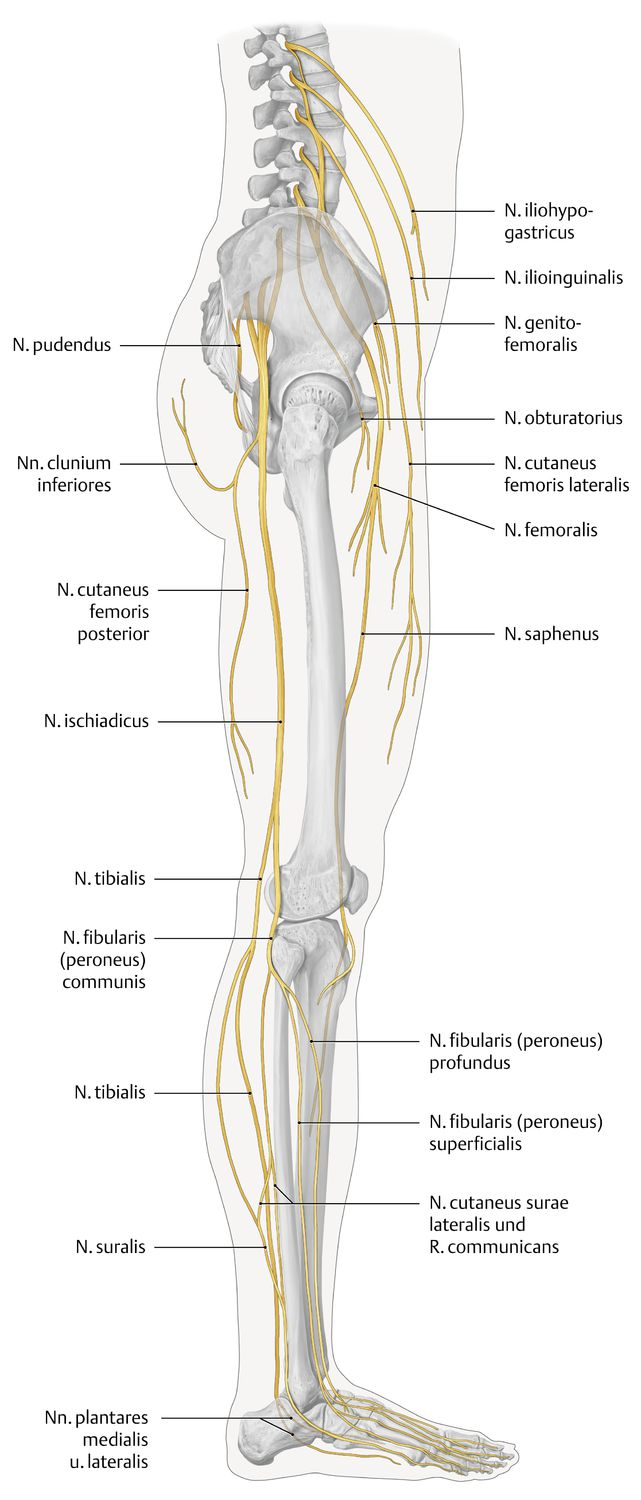
\includegraphics[width=\linewidth]{anat_sagittal}
            \label{fig:subfig:anat_sagittal}
        }
    \end{minipage}
    \begin{minipage}[c][0.9\textheight][t]{.5\textwidth}
        \centering
        \vspace*{\fill}
        \subfloat[]
        {
            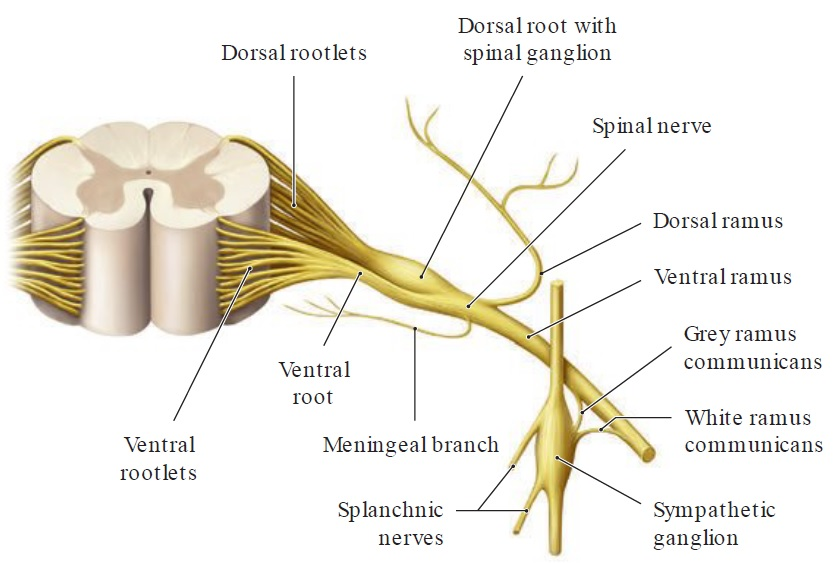
\includegraphics[width=\linewidth]{anat_spinal}
            \label{fig:subfig:anat_spinal}
        }
        \vfill
        \subfloat[]
        {
            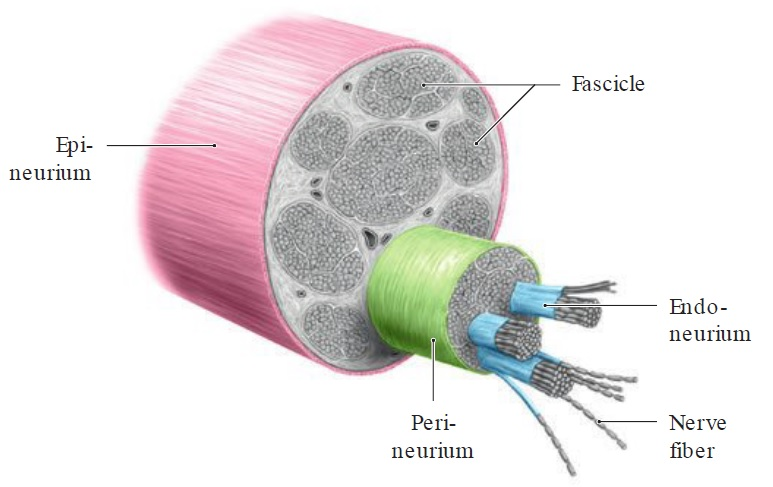
\includegraphics[width=\linewidth]{anat_nerve}
            \label{fig:subfig:anat_nerve}
        }
    \end{minipage}
    \vspace*{-0.3cm}
    \caption[Anatomy of the Peripheral Nervous System]{The anatomy of the \gls{pns} on different scales. \textbf{(a)} Nerves of the \gls{pns} of the lower limb, including \gls{n.} ischiadicus. \gls{n.} ischiadicus splits into \gls{n.} tibialis and \gls{n.} fibularis proximal to the knee. Image from~\cite{Schunke2014PrometheusAnatomie}. \textbf{(b)} Sensory nerves entering the spinal cord dorsal, motor nerves exiting the spinal cord ventral. Image from~\cite{Schunke2015THIEMEAnatomy} \textbf{(c)} Structure of a peripheral nerve. Image from~\cite{Schunke2015THIEMEAnatomy}.}
    \label{fig:anat}
\end{figure}

\begin{figure}[htbp]
	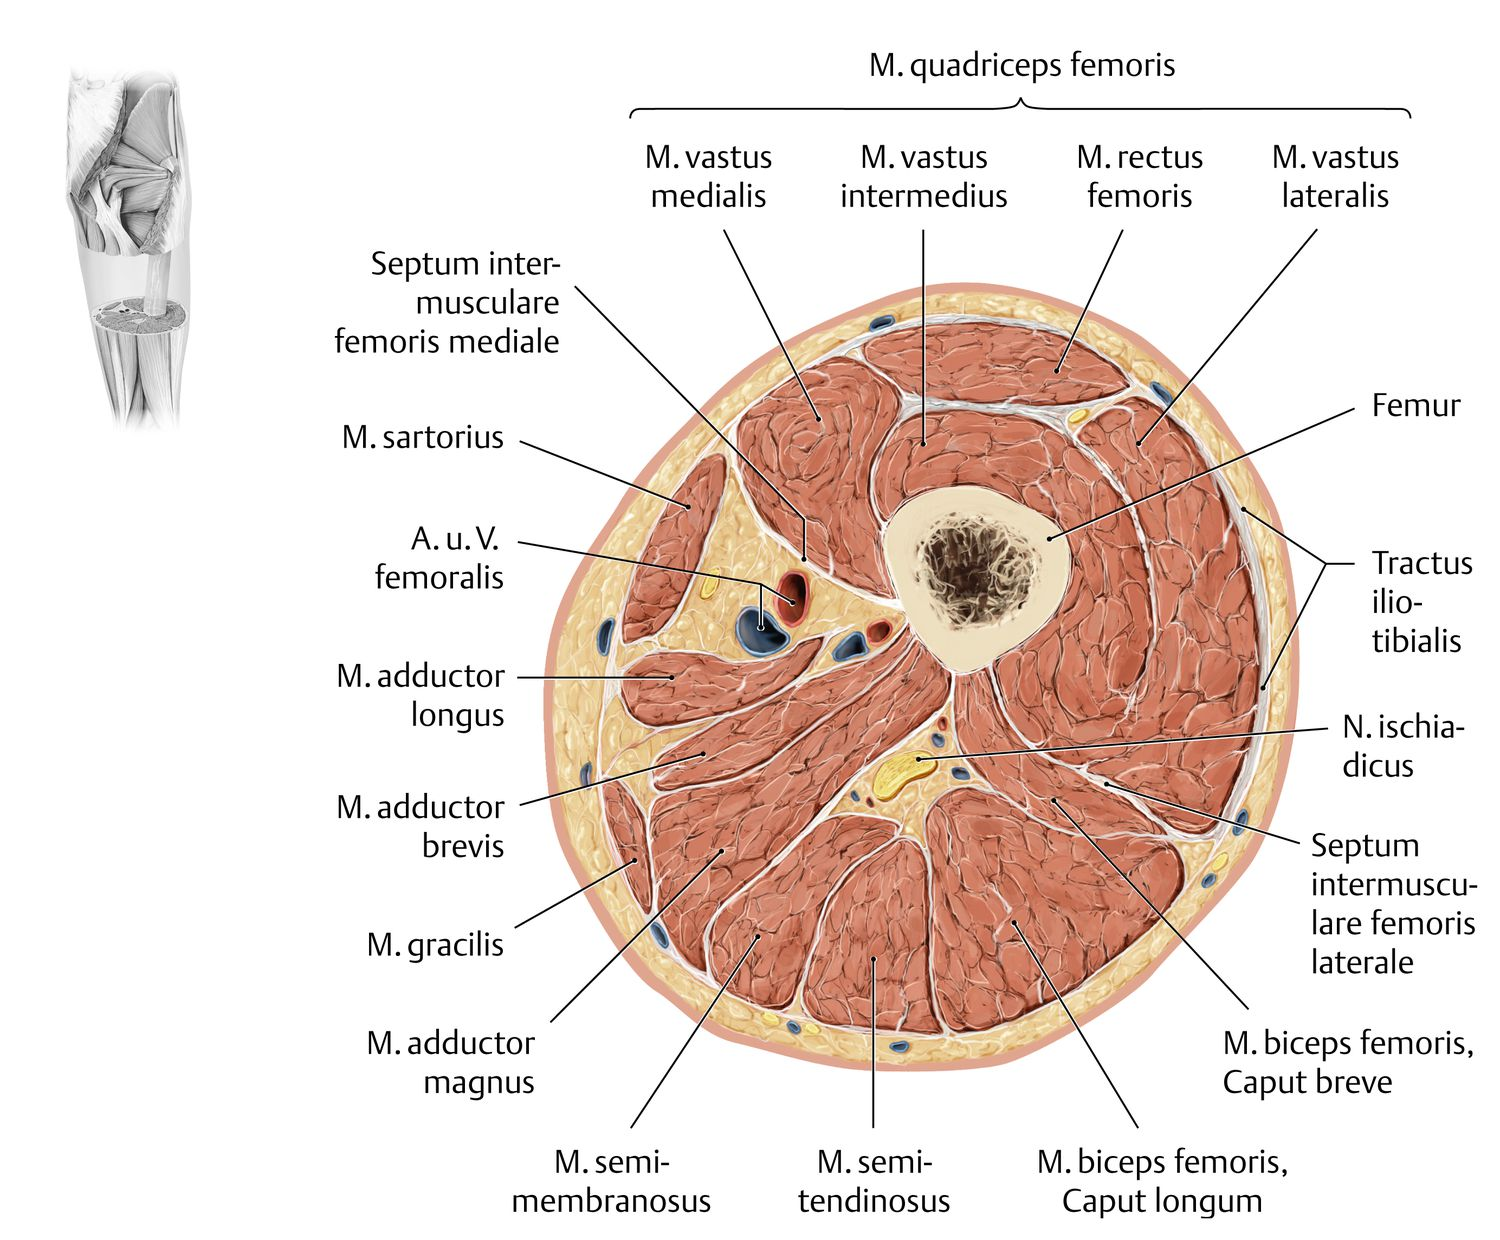
\includegraphics[width=\textwidth]{anat_axial}
    \caption[Cross-section of the Right Upper Leg]{Cross-sectional view of the right upper leg with femur, muscles, blood vessels and \gls{n.} ischiadicus. Image from~\cite{Schunke2014PrometheusAnatomie}.}
    \label{fig:anat_axial}
\end{figure}

\subsection{Peripheral Neuropathies}
The prevalence of peripheral neuropathies is approximatively 2.4 \% and rising to 8.0 \% with the age $\geq$ 55 years \cite{Martyn1997EpidemiologyNeuropathy}. The most common cause of peripheral neuropathies in the developed world is diabetes mellitus. Other causes include metabolic disorders, infections, toxins, and drugs \cite{England2004PeripheralNeuropathy,Hughes466}.
Peripheral neuropathies can be caused by the damage of the axons or by demyelination which hinders the fast transmission of neural signals. 
As the \gls{ans} controls almost every organ, a wide range of symptoms can arise when it is damaged. Damage to motor nerves may give rise to movement impairment or muscle weakness~\cite{Mohassel2015}. Damage to sensory nerves can be the cause of pain or altered sensation.

\subsection{State-of-the-Art Diagnosis}
\gls{eds} of the \gls{pns} are clinical tools that aid in the diagnostic assessment of patients with signs and symptoms of peripheral neuropathies~\cite{Mohassel2015}. \gls{eds} are used as an extension of the neurologic examination, and their primary goal is to help with localization of peripheral nerve lesions and find their distribution~\cite{Mohassel2015} (focal, multifocal, or generalized; one segment, multiple segments, or diffuse within the nerve). Additionally, \gls{eds} help determining age, severity, pathology, prognosis and can be used for treatment planning~\cite{Mohassel2015}. Many physiologic and non-physiologic factors, e.g., age, height, tissue temperature, and pathology influence \gls{eds}. Normally, \gls{eds} are composed of two different tests, which are related and complement each other.\\
\textbf{\gls{ncs}}: \gls{ncs} measure the electrical signal propagation along a given nerve. The nerve of interest is stimulated at one site, and the electrical response signal is measured at another and is analyzed. Correct stimulation of proximal and deeper nerves is difficult. Hence those nerves are typically hard to assess with \gls{ncs}~\cite{Mohassel2015}. Typical signal measurements for \gls{ncs} include distal latency, amplitude, conduction velocity, and late response latency. Prolonged distal and late response latency, and reduced conduction velocity can indicate degeneration of the myelin sheath. A decreased amplitude can be the indicator of axonal degeneration~\cite{Mohassel2015}.\\
\textbf{\gls{emg}}: \gls{emg} or needle {emg} complements \gls{ncs}, and can help confirm suspected pathologic processes. As \gls{emg} comes with discomfort for the patient, and a large number of muscles which could potentially be studied, it is important to have a detailed anatomical knowledge and a hypothesis-driven approach~\cite{Mohassel2015}. The \gls{emg} needle is an electrode that is directly inserted into the muscle and locally samples electrical activity of the muscle fibers. \gls{emg} includes evaluation of spontaneous activity at rest and the assessment of voluntary motor units upon activation~\cite{Mohassel2015}.
As of today \gls{eds} are the first choice for diagnosis of peripheral neuropathies. Apparent drawbacks are the insertion of the needle during \gls{emg} and that electrical stimulation may be painful or cause discomfort. Furthermore, \gls{eds} may not be applicable to nerves situated deep in the body or may yield inconclusive results.

\section{Medical Image Segmentation} \label{sec:intro_mia} % ===================================================================

\section{Machine Learning} \label{sec:intro_mlearn} % =============================================================================
In this part we briefly describe some fundamentals of machine learning. Machine learning is a huge topic and this section is by no means meant to be a complete overview. We only rather introduce some concepts and mention topics which were related and important for our work.

\subsection{Supervised Learning} \label{sec:ml_supervised}
The principle of supervised learning is illustrated on the prediction of house prizes as a function of their living area in Figure~\ref{fig:dl_supervised} taken from~\cite{Ng2012StanfordNotes}. In supervised learning, we train an algorithm (or also called model) by showing the algorithm input-output pairs (e.g., living area of houses versus their corresponding prizes). This is referred to as the training phase, and the input-output pairs are called the training set. The outputs are typically referred to as labels or targets. More formally we define the training set as
\begin{equation}
   S_{Train} = \{(x^{(i)}, y^{(i)}); i = 1,...,m\}
   \label{eq:training_set}
\end{equation}
and let $\chi$ and $\upsilon$ denote the space of input and output values, respectively. In this example, $\chi = \upsilon = \mathbb{R}$. The aim of the training phase is to let the algorithm (hopefully) learn a meaningful relationship between the inputs and outputs of our training set. Therefore, we aim learn a mapping $h : \chi \mapsto \upsilon$, parameterized by a set of models weights~$\textbf{W}$, which is "good" for all pairs in $S_{Train}$, hence
\begin{equation}
   y^{(i)} = h(x^{(i)}, \mathbf{W}); i = 1,...,m
   \label{eq:model}
\end{equation}
is approximatively valid for all training pair. We call $h(x^{(i)}, \mathbf{W})$ our model with the model weights~$\textbf{W}$. Depending on the on the type of mapping, $\mathbf{W}$ is typically a Matrix and we therefore, write it in bold font. If the learned relation is correct, the model can be used to make predictions on previously unseen input data.\\
If the output, we are trying to predict, is continuous, such as in the housing example, the problem is called a \textbf{regression problem}. We could also have the case where we wanted to predict whether the dwelling is an apartment or a house, given the living area. The predicted output would, therefore, be discrete and we would call this a \textbf{classification problem}.\\
Supervised learning gets its name for the reason that the algorithm always learns on input-output pairs (the outputs typically called labels or targets), and the outputs typically are the result of (laborsome) labeling work done by a person. This is the biggest drawback of supervised learning. There, however, exist ways to use unlabeled data in conjunction with labeled data, referred to as semi-supervised learning. Learning on inputs only corresponds to finding patterns and structures in the input space and is referred to as unsupervised learning. Typical examples for unsupervised learning algorithms are \gls{pca} and $k$-means Clustering~\cite{Goodfellow2016DeepLearning}.\\
For the presented example, one could expect a linear relationship, between the living area of a house and its prize. If this was indeed true, we could make robust predictions with a simple linear model, i.e. $y^{(i)} = h(x^{(i)}, W) = Wx^{(i)} + b$, only incorporating the living area. However, one could argue that the number of rooms or the location, each with its unknown weight, also influence the dwelling's prize. These influencers are typically called features. There was, and still, is a whole science around finding good features to solve learning problems.\\
The main drawback of any learning algorithm relying on features is, however, that the algorithm is inherently constrained by the imagination and ability of the engineer to find and implement good features.

\begin{figure}[htbp]
    \centering
	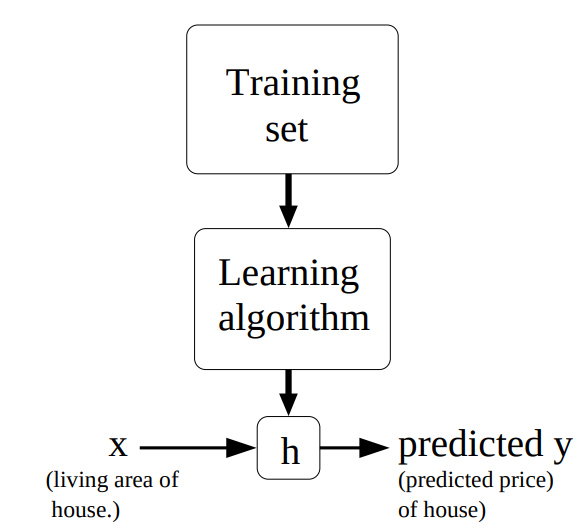
\includegraphics[width=0.5\textwidth]{supervised_learning}
    \caption[Supervised Learning]{The principle of supervised learning illustrated on the example of predicting house prices (y) depending on the living area (x). Suppose we have $m$ area-price pairs, which we name our training set: $\{(x^{(i)}, y^{(i)}); i = 1,...,m\}$. We let $\chi$ and $\upsilon$ denote the space of input and output values, respectively. In this example, $\chi = \upsilon = \mathbb{R}$. In supervised learning we aim to learn a function (also called mapping) $h : \chi \mapsto \upsilon$, which makes reasonable prize prediction (y) for a given new house area (x). We use the training set to learn $h$. Image and example taken from~\cite{Ng2012StanfordNotes}.}
    \label{fig:dl_supervised}
\end{figure}

\subsection{Training}
In the previous section we defined that the model $h(x^{(i)}, \mathbf{W})$ is parameterized by the set of weights $\textbf{W}$. During the training phase of the model, we adjust $\textbf{W}$ in order for the model to make "better" predictions on the training set. Formally, we want to solve the optimization problem
\begin{equation}
   \mathbf{W}^{*} = \argmin_\textbf{W} \sum_{i=1}^{m} L(h(x^{(i)}, \mathbf{W}), y^{(i)})
   \label{eq:optimization}
\end{equation}
where $L(...)$ denotes a loss function. The loss function is a metric we have to choose, which calculates the error between the correct label $y^{(i)}$ and the prediction our model made. The loss function is often also referred to as cost function. $\mathbf{W}^{*}$ denotes the solution for the mentioned optimization problem and, consequently, is the set of weights which results in the smallest error in our training set. Training of a model corresponds to iteratively decreasing the training error.\\
A loss function typically used for classification problems with $k$ classes, a prediction vector $\mathbf{h}^{(i)}$ and label vector $\mathbf{y}^{(i)}$, is the \textbf{cross-entropy} loss

\begin{equation}
    L(\mathbf{h}^{(i)}, \mathbf{y}^{(i)}) = -\mathbf{y}^{(i)} \log(f(\mathbf{h}^{(i)}))
    \label{eq:cross_entropy_multi}
\end{equation}
with $f(...)$ being the \textbf{softmax} activation function
\begin{equation}
   f(\mathbf{h}^{(i)}) = \frac{\exp\mathbf{h}^{(i)}}{\sum_{j} \exp{\mathbf{h}^{(i)}_{j}}}
   \label{eq:softmax}
\end{equation}
which squashes the predictions into a vector of values between zero and one that add up to one. The corresponding cross-entropy loss for a binary classification problem
\begin{equation}
    L({h}^{(i)}, {y}^{(i)}) = -{y}^{(i)} \log(\sigma({h}^{(i)}))
    \label{eq:cross_entropy_binary}
\end{equation}
with $\sigma(...)$ being the \textbf{sigmoid} activation function
\begin{equation}
   \sigma({h}^{(i)}) = \frac{1}{1 + \exp{(-{h}^{(i)})}}
   \label{eq:sigmoid}
\end{equation}
Another, in deep learning very popular, activation function is the \textbf{\gls{relu}}, defined as
\begin{equation}
   ReLU({h}^{(i)}) = \max(0, {h}^{(i)})
   \label{eq:relu}
\end{equation}

In order to solve Equation~\ref{eq:optimization}, optimizer are used. Optimizer, such as \gls{sgd}~\cite{Goodfellow2016DeepLearning} and Adam~\cite{Kingma2014Adam:Optimization} use the gradient to find $\textbf{W}^*$. The gradient depends on the model and the chosen loss function and corresponds the first order derivative of the individual inputs with respect to the output.\\

A common problem in machine learning, especially in deep learning, is the problem of under- and overfitting, which is depicted in Figure~\ref{fig:under_over_fitting}. To solve a learning problem, we have to choose a model first. The model's representational power, hence the ability to fit a wide variety of functions, is called capacity~\cite{Goodfellow2016DeepLearning}. If the models capacity is too low for the task at hand, it cannot model the relationship between the input and output. This is called underfitting. On the other hand, if the models capacity is too high, it can start to memorize the data it was trained upon (including the data's statistics) rather than learning structures or relationships. This results in a bad performance on new data, hence bad generalization and is called overfitting.

\begin{figure}[htbp]
    \centering
	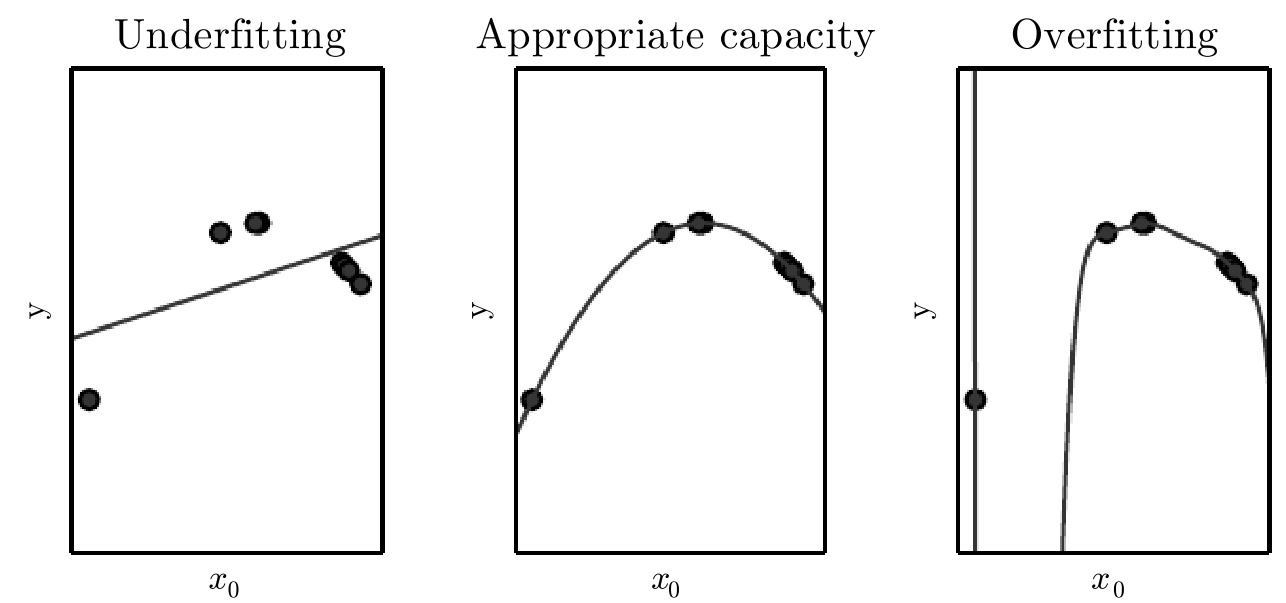
\includegraphics[width=0.8\textwidth]{under_over}
    \caption[Under- and Overfitting]{The problem of under- and overfitting. The sample points were generated by random sampling a quadratic function. In the left image, a model with low capacity (a line) is not able to correctly capture the structure of the points. The center image shows that a quadratic model would generalize well to unseen ponts. The right image shows that a 9\textsuperscript{th} degree polynomial would generalize bad to new points despite passing through all points. Image and example taken from~\cite{Goodfellow2016DeepLearning}.}
    \label{fig:under_over_fitting}
\end{figure}

\subsection{Deep Learning \& Convolutional Neural Networks}
With the growing amount of labeled data, gathered in big datasets, and increasing computational performance using \gls{gpu}'s, the creation and training of models, called neural networks, with much larger capacity became possible. Today, some of the biggest datasets for images are ImageNet~\cite{Russakovsky2015ImageNetChallenge} and Microsoft's COCO~\cite{Lin2014MicrosoftContext}.
Neural networks
The most significant advantage of those models was that (given enough training data) it was now possible to train them directly on raw, unprocessed data, rather than on human-engineered features.\\
\gls{cnn}s, a class of neural network mostly used to analyze visual imagery, were successfully applied \cite{Lecun2015DeepLearning} and achieved new levels of performances in computer vision tasks and challenges \cite{Krizhevsky2012ImageNetNetworks,Simonyan2014VeryRecognition,Szegedy2014GoingConvolutions,He2015DeepRecognition,Zeiler2014VisualizingNetworks}. 
\gls{cnn}s and neural networks in general, use a cascade of multiple layers of units which can process
and transform data. Each layer takes the previous layer's output as an input. \gls{cnn}s, in contrast to regular neural networks, assume that the input data has some spatial relationship, hence the popular use of \gls{cnn}s for computer vision tasks. Because a \gls{cnn} consists of several sequential convolutional layers, the learned filters deeper in the network can act as detectors for higher semantical features. Therefore it can learn multiple levels of representations, which correspond to multiple levels of abstraction. During training, a \gls{cnn} learns filters which act as detectors for features which are present in the data. It basically builds its internal filter bank to extract information. Figure~\ref{fig:mlearn_weights} shows the learned filters in the first layer of an AlexNet which was trained on ImageNet~\cite{Russakovsky2015ImageNetChallenge}. Note that the learned weights resemble filters for edge or blob detection (sobel operator~\cite{Sobel1990AnOperator}, laplacian of gaussian~\cite{Marr187}) widely used in computer vision.\\

A typical \gls{cnn} is built as a sequence of multiples of the following layers~\cite{KarpathyStanfordRecognition}. Each layer transforms the activations of the previous layer into new activations, through a differentiable function.\\
\textbf{Convolutional Layer:} Layer which contains the learnable weights. The learnable weights form filters, which are used for information extraction. Parameters for a convolutional layer are typically the kernel size of the filters and the number of individual filters (also referred to as channels or features).\\
\textbf{ReLU Layer:} Applies the Equation~\ref{eq:relu} to each of the outputs of the previous layer. This results in thresholding at zero. Other typical activation functions are the sigmoid (Equation~\ref{eq:sigmoid}) or tanh function.\\
\textbf{Pooling Layer:} A pooling layer performs a down-sampling operation along the spatial dimensions. Typically max-pooling is used, which only lets the maximum activation through. Pooling helps prevent overfitting by reducing the number of parameters in a network.\\
\textbf{Transposed Convolutional Layer:} A transposed convolutional layer performs and up-sampling operation along the spatial dimensions and is typically used as the inverse operation of the pooling layer.\\
\textbf{Dropout layer:} Randomly deactivates some of the activations of the previous layer. Dropout~\cite{Srivastava2014Dropout:Overfitting} helps with the overfitting problem.\\
\textbf{Normalization Layer:} Different types of normalization layers have been proposed, including Batch Normalization~\cite{SergeyIoffe2015BatchNormalization}. They all normalize of the activations in some way.
 
\begin{figure}[htbp]
	\centering
	\subfloat[]
	{
		\label{fig:subfig:mlearn_nn}
		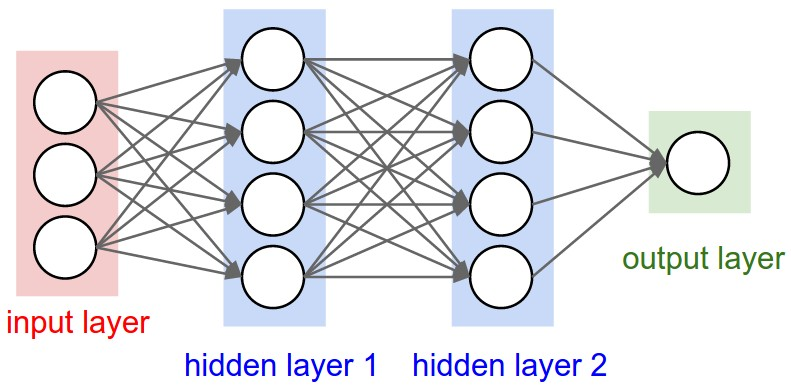
\includegraphics[width=0.48\textwidth]{mlearn_neural_network}
	}
	\hfill
	\subfloat[]
	{
		\label{fig:subfig:mlearn_cnn}
		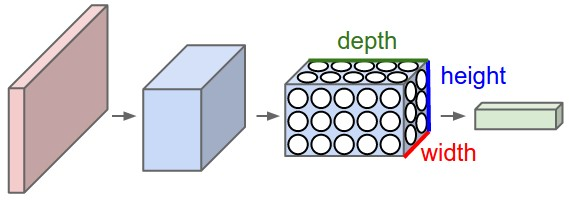
\includegraphics[width=0.48\textwidth]{mlearn_cnn}
	}
	\caption[Sections of MRN sequences]{\textbf{(a)} Regular neural network where each node of a layer is connected to every node of the previous. \textbf{(b)} CNN where the weights are organized in a \gls{3d} way. Each of the nodes is only locally connected to nodes of the previous layer. The main motivation behind this is that a learned filter (e.g. edge detector) is useful over the whole image. Both Images are from~\cite{KarpathyStanfordRecognition}.}
	\label{fig:mlearn_nn_cnn}  
\end{figure}


\begin{figure}[htbp]
    \centering
	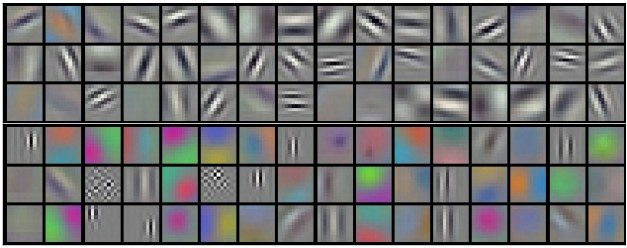
\includegraphics[width=0.8\textwidth]{mlearn_weights}
    \caption[Learned Weights of trained AlexNet]{Learned convolutional filters of the first layer of an AlexNet~\cite{Krizhevsky2012ImageNetNetworks} which was trained on ImageNet. The learned filters act as detectors for high-frequency grayscale features, mostly edges, and low-frequency color features.}
    \label{fig:mlearn_weights}
\end{figure}



\section{Related Work} % =================================================================================

This is precisely what F. Balsiger did during his master thesis~\cite{Balsiger2016DevelopmentApproaches}: He investigated the different impact features had on the segmentation results of the peripheral nerves done by a trained \gls{rf}~\cite{Breiman2001RandomForests}. The \gls{rf}, also belonging to supervised learning, was trained by engineered features calculated on the \gls{mrn} images. This resulted in a voxel-wise classification into the labels \textit{peripheral nerve} and \textit{background}, hence a segmentation of the peripheral nerves. \\

\section{Hypothesis} % ===================================================================================

\textit{Deep-learning-based segmentation of peripheral nerves from \gls{mrn} images is possible.} \\
\textit{3D-Contextual information allows for better segmentation results.}

\section{Aim \& Structure of the Thesis} % ===============================================================

\endinput